\documentclass{article}
\usepackage[yyyymmdd]{datetime}
\usepackage[shortlabels]{enumitem}
\usepackage[nottoc]{tocbibind}
\usepackage{url}
\usepackage{float}
\usepackage[margin=1in]{geometry}
\usepackage{xcolor}
\usepackage{mdframed}
\usepackage{amsfonts}
\usepackage{amsmath}
\usepackage{amssymb}
\usepackage{amsthm}
\usepackage{tikz}
\usepackage{pgfplots}
\usepackage{graphicx}
\graphicspath{{./images}}


\pgfplotsset{width=10cm,compat=1.9}
\usepgfplotslibrary{external}
\definecolor{pearl}{RGB}{234,224,220}
\definecolor{bg-se}{RGB}{246, 246, 246}
\usepackage{listings}

\definecolor{clr-background}{RGB}{255,255,255}
\definecolor{clr-text}{RGB}{0,0,0}
\definecolor{clr-string}{RGB}{163,21,21}
\definecolor{clr-namespace}{RGB}{0,0,0}
\definecolor{clr-preprocessor}{RGB}{128,128,128}
\definecolor{clr-keyword}{RGB}{0,0,255}
\definecolor{clr-type}{RGB}{43,145,175}
\definecolor{clr-variable}{RGB}{0,0,0}
\definecolor{clr-constant}{RGB}{111,0,138} % macro color
\definecolor{clr-comment}{RGB}{0,128,0}

\lstdefinestyle{VS2017}{
	backgroundcolor=\color{white},
	basicstyle=\color{clr-text}, % any text
	stringstyle=\color{clr-string},
	identifierstyle=\color{clr-variable}, % just about anything that isn't a directive, comment, string or known type
	commentstyle=\color{clr-comment},
	directivestyle=\color{clr-preprocessor}, % preprocessor commands
	% listings doesn't differentiate between types and keywords (e.g. int vs return)
	breakatwhitespace=false,         
	breaklines=true, 
	% use the user types color
	keywordstyle=\color{clr-type},
	keywordstyle={[2]\color{clr-constant}}, % you'll need to define these or use a custom language
	tabsize=2
}

% Make header with name and date etc.
\usepackage{fancyhdr}
\lhead{Pedro D. Llerenas\\An\'alisis de Datos I}
\rhead{\today\\Tarea I}
\thispagestyle{fancy}

\usepackage[utf8]{inputenc}
\setlength{\parindent}{0pt} % Don't indent new paragraphs
\setlength{\headheight}{24pt} 

\newcommand{\Z}{{\mathbb Z}}
\newcommand{\N}{\mathbb N}
\newcommand{\Q}{\mathbb Q}
\newcommand{\R}{\mathbb R}
\newcommand{\C}{\mathbb C}


\begin{document}
<<<<<<< HEAD

\begin{enumerate}


	\item Como es bien sabido, la representaci\'on num\'erica binaria de tipo signo/exponente/mantisa, depende de la creatividad o precisi\'on que desee el programador. Analicemos qu\'e sucede con un sistema de numeraci\'on binario a $n>0$ (entero) bits, para esto elige un valor par entre 10 y 20, crea el sistema de numeraci\'on entero similar al estudiado en clase, (la mantisa debe ser, al menos, la mitad del n\'umero elegido). Describe tu sistema de numeraci\'on, ¿Cu\'al es el menor y mayor de los n\'umeros representados? Presenta un n\'umero que no se pueda representar en tu sistema seleccionado. Describe tu proceso. (4 pts) NOTA: punto extra si adem\'as se describe un sistema fraccionario que tenga sentido.
	      \begin{mdframed}[
			      linecolor=darkgray,
			      backgroundcolor=white]
		      \begin{proof}[\textbf{Demostraci\'on.}]
			      Usaremos 16 bits en total. 1 para el signo, 3 para el exponente, 12 para la mantisa. Esto nos genera n\'umeros en el rango
			      \[ [-1*2^7*(2^{12} - 1), 2^7*(2^{12} - 1)] = [-524160, 524160] \]

			      \lstinputlisting[caption=Calcular epsilon de la m\'aquina, language=C, style=VS2017]{p1.c}


			      el c\'odigo anterior genera un csv con todos los valores (positivos) posibles de la representaci\'on elegida.

			      Para el sistema fraccionario, definimos el bit implicito como

			      $$
				      \begin{cases}
					      \texttt{b}_{imp}= 1   & \texttt{if } 0 <\texttt{exp} < 7                           \\
					      \texttt{b}_{imp} =  0 & \texttt{if } \texttt{exp} = 0 \texttt{ and matissa} \neq 0
				      \end{cases}
			      $$
			      y
			      $$
				      \begin{cases}
					      \texttt{exp}=\texttt{exp}-3 & \texttt{if } 0 <\texttt{exp} < 7 \\
					      \texttt{exp} = 2            & \texttt{if } \texttt{exp} = 0
				      \end{cases}
			      $$
			      de esta manera, obtenemos los valores que

		      \end{proof}
	      \end{mdframed}

	\item Consideremos la siguiente sucesi\'on $\{x_n\}_{n\in \N} \subset \R$ definida de manera recurrente como: (4 pts)
	      \begin{align*}
		      x_2     & =2,                                               \\
		      x_{n+1} & = 2^{n-\frac{1}{2}}\sqrt{1-\sqrt{1-4^{1-n}x^2_n}}
	      \end{align*}
	      \begin{enumerate}
		      \item Escribe un programa para encontrar los primeros $n$ t\'erminos de la sucesi\'on.
		      \item Aplica tu programa para encontrar los t\'erminos de la sucesi\'on cuando $$n = 6, 7, 8, 9, 10,12, 18, 20$$, ¿a qu\'e valor tiende la sucesi\'on? (\'esta sucesi\'on tiende a un valor distinto de cero).
		      \item Encuentra los t\'erminos 50 y 100, ¿qu\'e sucede con la sucesi\'on? Grafica los t\'erminos de la sucesi\'on desde 2 hasta 100. Explica detalladamente el por qu\'e del comportamiento que tiene la computadora al calcular estos t\'erminos.
	      \end{enumerate}
	      \begin{mdframed}[
			      linecolor=darkgray,
		      ]
		      \begin{proof}[\textbf{Demostraci\'on.}]
            Primero mostraremos que utilizar directamente la secuencia resulta en los t\'erminos divergiendo a infinito debido a los errores de precisi\'on de punto flotante. 
            Podemos notar que la secuencia puede ser reescrita de tal manera que la cantidad de restas (2) se puede reducir a 1. 
            \begin{align*}
              x_{n+1} &= 2^{n-1/2} \sqrt{1-\sqrt{1-4^{1-n}x^2_n}}\\
                     &= 2^{n-1/2} \sqrt{1-\sqrt{1-4^{1-n}x^2_n}} \cdot\frac{\sqrt{1-\sqrt{1+4^{1-n}x^2_n}}}{\sqrt{1+\sqrt{1-4^{1-n}x^2_n}}}\\
                     &= 2^{n-1/2}\frac{\sqrt{1-(1-4^{1-n}x^2_n)}}{\sqrt{1-\sqrt{1+4^{1-n}x^2_n}}} \\
                     &= 2^{n-1/2} \frac{2^{1-n}x_n}{\sqrt{1-\sqrt{1+4^{1-n}x^2_n}}}\\
                     &= \frac{\sqrt{2}x_n}{\sqrt{1-\sqrt{1+4^{1-n}x^2_n}}}.
            \end{align*}
			      \lstinputlisting[caption=Calcular secuencia de n\'umeros que se acerca a $\pi$, language=C, style=VS2017]{p2.c}

            \begin{figure}[H]
             \caption{Secuencia usando algoritmo ingenuo}
				      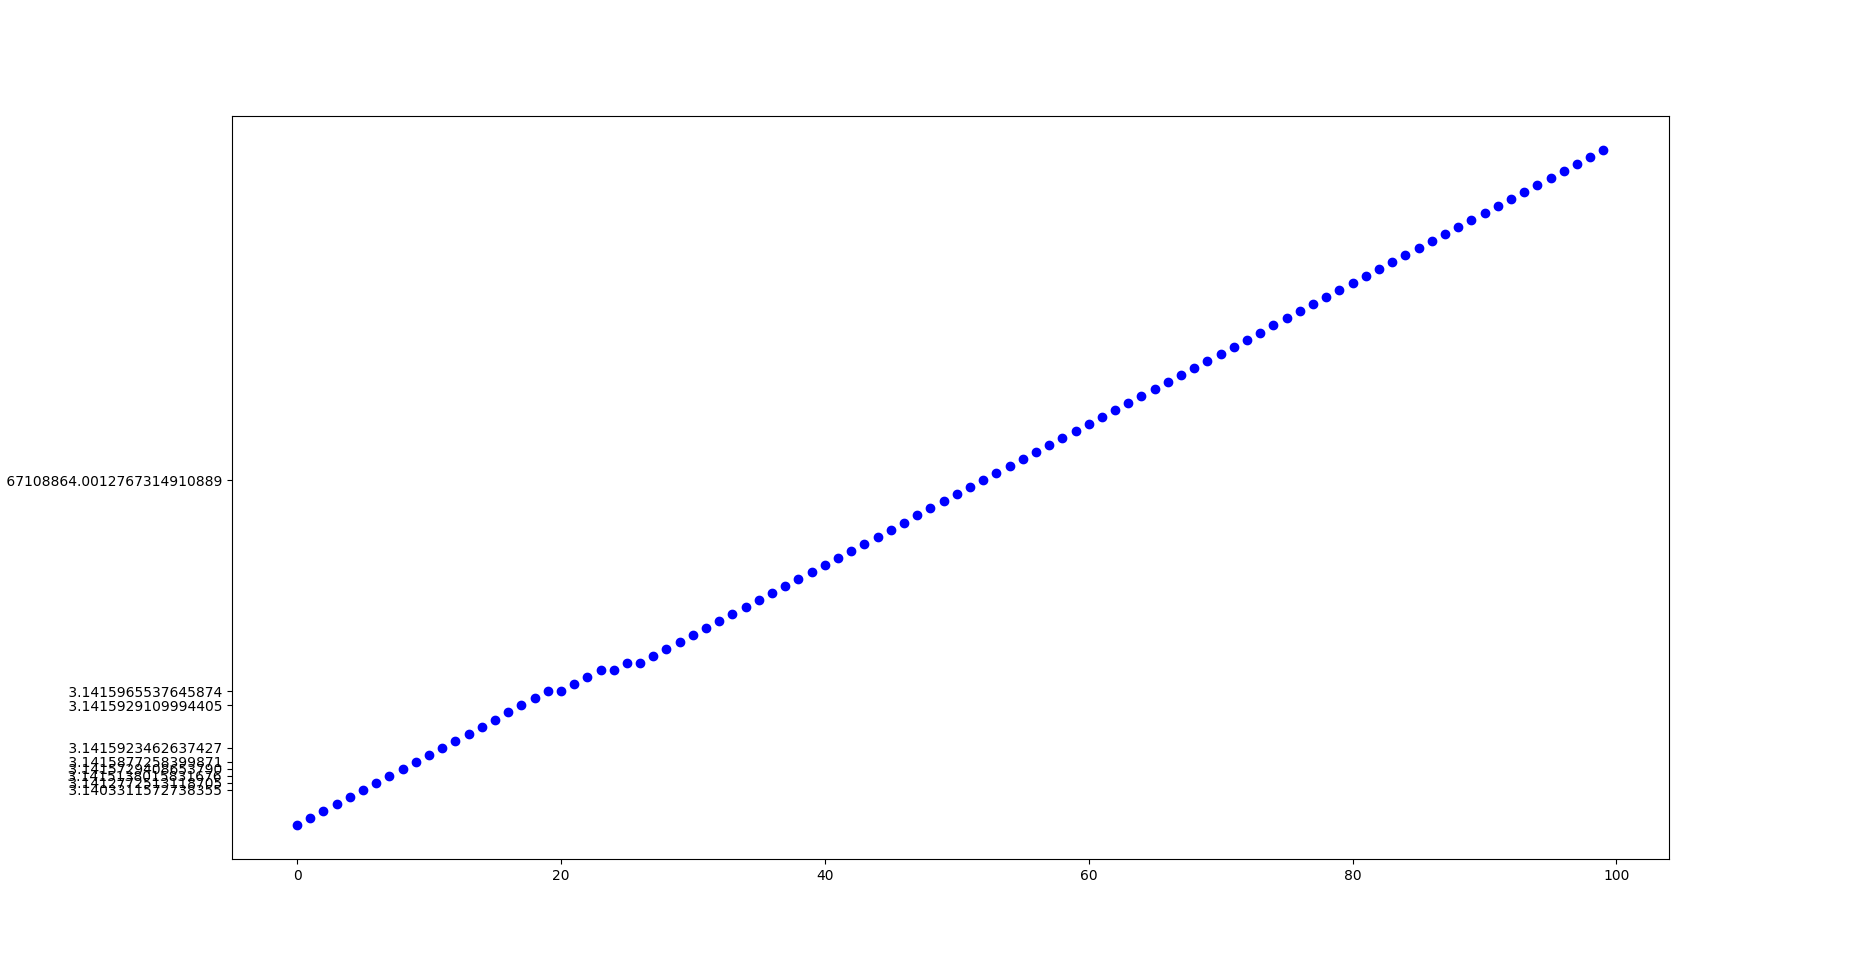
\includegraphics[width=\textwidth]{naive_pi_approx}
            \end{figure}

            \begin{figure}[H]
             \caption{Secuencia usando algoritmo reduciendo restas}
				      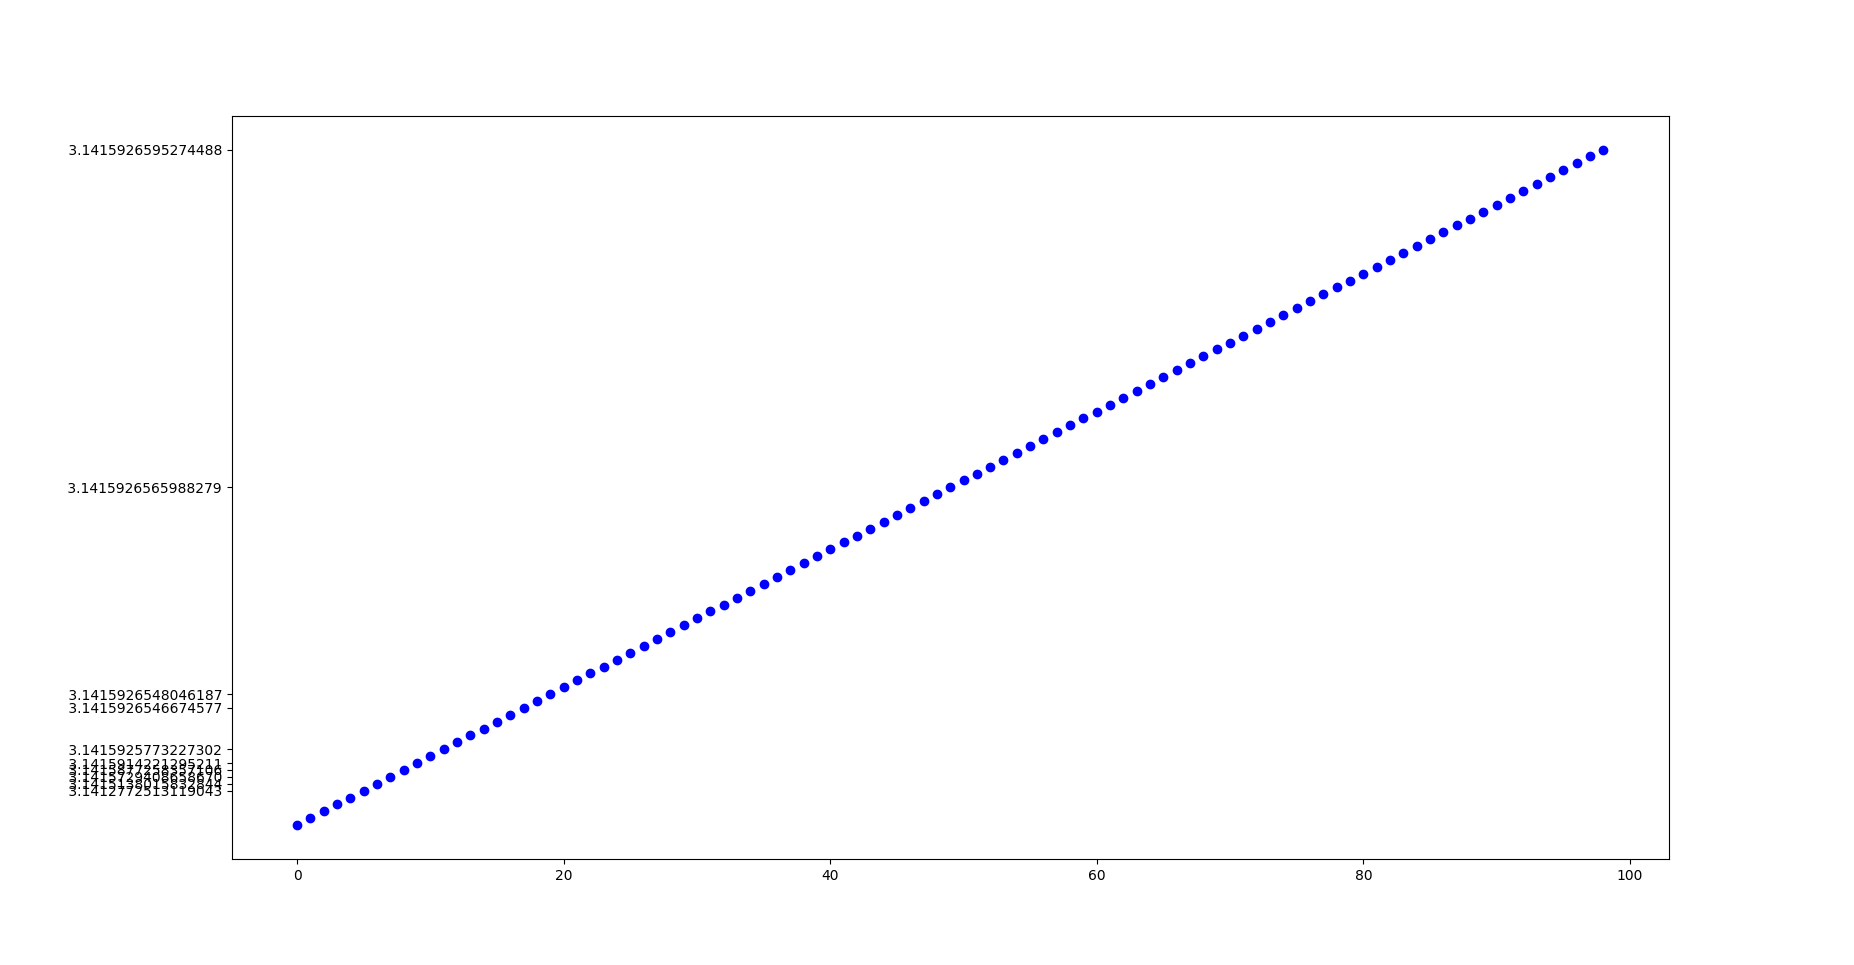
\includegraphics[width=\textwidth]{pi_approx}
            \end{figure}
              
            Como podemos observar, el segundo algoritmo (que reduce el numero de restas), se mantiene cerca de $\pi$, mientras que el ingenuo explota y diverge a infinito.
		      \end{proof}
	      \end{mdframed}


	\item Al n\'umero representable inmediatamente despu\'es de la unidad se le conoce como el epsil\'on de la computadora
	      machine el cual nos permite calcular el n\'umero real representable inmediatamente posterior; \'esto se obtiene
	      al multiplicar el epsil\'on por el real y sumarlo a ese real. Utilizando el siguiente algoritmo, crea un c\'odigo
	      que calcule el machine de tu computadora, s\'olo hace falta indicar el tipo de variable que es "epsilon" (float o
	      doble). El \'ultimo valor impreso corresponde al epsilon de la computadora. (2 pts)
	      \begin{mdframed}[
			      linecolor=darkgray,
			      backgroundcolor=white]
		      \begin{proof}[\textbf{Demostraci\'on.}]
			      La lista impresa es
			      \begin{center}

				      1.0000000000000000000000\\
				      0.5000000000000000000000\\
				      0.2500000000000000000000\\
				      0.1250000000000000000000\\
				      0.0625000000000000000000\\
				      0.0312500000000000000000\\
				      0.0156250000000000000000\\
				      0.0078125000000000000000\\
				      0.0039062500000000000000\\
				      0.0019531250000000000000\\
				      0.0009765625000000000000\\
				      0.0004882812500000000000\\
				      0.0002441406250000000000\\
				      0.0001220703125000000000\\
				      0.0000610351562500000000\\
				      0.0000305175781250000000\\
				      0.0000152587890625000000\\
				      0.0000076293945312500000\\
				      0.0000038146972656250000\\
				      0.0000019073486328125000\\
				      0.0000009536743164062500\\
				      0.0000004768371582031250\\
				      0.0000002384185791015625\\
				      0.0000001192092895507812\\
				      0.0000000596046447753906\\
				      0.0000000298023223876953\\
				      0.0000000149011611938477\\
				      0.0000000074505805969238\\
				      0.0000000037252902984619\\
				      0.0000000018626451492310\\
				      0.0000000009313225746155\\
				      0.0000000004656612873077\\
				      0.0000000002328306436539\\
				      0.0000000001164153218269\\
				      0.0000000000582076609135\\
				      0.0000000000291038304567\\
				      0.0000000000145519152284\\
				      0.0000000000072759576142\\
				      0.0000000000036379788071\\
				      0.0000000000018189894035\\
				      0.0000000000009094947018\\
				      0.0000000000004547473509\\
				      0.0000000000002273736754\\
				      0.0000000000001136868377\\
				      0.0000000000000568434189\\
				      0.0000000000000284217094\\
				      0.0000000000000142108547\\
				      0.0000000000000071054274\\
				      0.0000000000000035527137\\
				      0.0000000000000017763568\\
				      0.0000000000000008881784\\
				      0.0000000000000004440892\\
				      0.0000000000000002220446\\

			      \end{center}

			      Despu\'es de 52 iteraciones, obtenemos que $$\epsilon = 0.0000000000000002220446 = 2.22046\times10^{-16} \approx 2^{-52}$$.
			      \lstinputlisting[caption=Calcular epsilon de la m\'aquina, language=C, style=VS2017]{p3.c}
		      \end{proof}
	      \end{mdframed}

\end{enumerate}
=======
	
	\begin{enumerate}
		
		
		\item Como es bien sabido, la representaci\'on num\'erica binaria de tipo signo/exponente/mantisa, depende de la creatividad o precisi\'on que desee el programador. Analicemos qu\'e sucede con un sistema de numeraci\'on binario a $n>0$ (entero) bits, para esto elige un valor par entre 10 y 20, crea el sistema de numeraci\'on entero similar al estudiado en clase, (la mantisa debe ser, al menos, la mitad del n\'umero elegido). Describe tu sistema de numeraci\'on, ¿Cu\'al es el menor y mayor de los n\'umeros representados? Presenta un n\'umero que no se pueda representar en tu sistema seleccionado. Describe tu proceso. (4 pts) NOTA: punto extra si adem\'as se describe un sistema fraccionario que tenga sentido.
		\begin{mdframed}[
			linecolor=darkgray,
			backgroundcolor=pearl]
			\begin{proof}[\textbf{Demostraci\'on.}]
				Usaremos 16 bits en total. 1 para el signo, 3 para el exponente, 12 para la mantisa. Esto nos genera n\'umeros en el rango
				\[ [-1*2^7*(2^{12} - 1), 2^7*(2^{12} - 1)] = [-524160, 524160] \]
			\end{proof}
		\end{mdframed}
		
		\item Consideremos la siguiente sucesi\'on $\{x_n\}_{n\in \N} \subset \R$ definida de manera recurrente como: (4 pts)
		\begin{align*}
			x_2&=2,\\
			x_{n+1} &= 2^{n-\frac{1}{2}}\sqrt{1-\sqrt{1-4^{1-n}x^2_n}}
		\end{align*}
		\begin{enumerate}
			\item Escribe un programa para encontrar los primeros $n$ t\'erminos de la sucesi\'on.
			\item Aplica tu programa para encontrar los t\'erminos de la sucesi\'on cuando $n = 6, 7, 8, 9, 10, 12, 18, 20$, ¿a qu\'e valor tiende la sucesi\'on? (\'esta sucesi\'on tiende a un valor distinto de cero).
			\item Encuentra los t\'erminos 50 y 100, ¿qu\'e sucede con la sucesi\'on? Grafica los t\'erminos de la sucesi\'on desde 2 hasta 100. Explica detalladamente el por qu\'e del comportamiento que tiene la computadora al calcular estos t\'erminos.
		\end{enumerate}
		\begin{mdframed}[
			linecolor=darkgray,
			backgroundcolor=pearl]
			\begin{proof}[\textbf{Demostraci\'on.}]
				Para eficientizar los calculos, guardamos el \'ultimo valor de la sucesi\'on y algunas otras constantes que consisten de una operaci\'on b\'asica. 
        Notemos que adem\'as, podemos reescribir el t\'ermino para evitar restas. Esto nos permite reducir los errores acumulados.
				\lstinputlisting[caption=Calcular epsilon de la m\'aquina, language=C, style=VS2017]{p2.c}
			\end{proof}
		\end{mdframed}
		
		
		\item Al n\'umero representable inmediatamente despu\'es de la unidad se le conoce como el epsil\'on de la computadora
		machine el cual nos permite calcular el n\'umero real representable inmediatamente posterior; \'esto se obtiene
		al multiplicar el epsil\'on por el real y sumarlo a ese real. Utilizando el siguiente algoritmo, crea un c\'odigo
		que calcule el machine de tu computadora, s\'olo hace falta indicar el tipo de variable que es "epsilon" (float o
		doble). El \'ultimo valor impreso corresponde al epsilon de la computadora. (2 pts)
		\begin{mdframed}[
			linecolor=darkgray,
			backgroundcolor=pearl]
			\begin{proof}[\textbf{Demostraci\'on.}]
				Despu\'es de 52 iteraciones, obtenemos que $$\epsilon = 0.0000000000000002220446 = 2.22046\times10^{-16} \approx 2^{-52}$$.
				\lstinputlisting[caption=Calcular epsilon de la m\'aquina, language=C, style=VS2017]{p3.c}
			\end{proof}
		\end{mdframed}
		
	\end{enumerate}
>>>>>>> e754a4e (notes)
\end{document}
